\thispagestyle{myheadings} % should I be including this at the top of every section page??

\graphicspath{ {Body/Figures/Theory/} }

\chapter{Introduction}
\label{chapter:Introduction}

While the prevailing theory for particle physics, the Standard Model (SM), has had tremendous success in describing our universe, there exist unanswered questions. These namely include the matter-antimatter asymmetry, the source of mass for the neutrinos, the existance of dark matter, and more. Many particle physics experiments are being conducted around the world in order to shed light on these questions and round out our understanding of reality. One such particular experiment being conducted is the Fermilab Muon \gmtwo Experiment (E989) underway at the Fermi National Accelerator Laboratory (FNAL) located in Batavia, Illinois. It has the goal of measuring the magnetic moment of the muon, proportional to the $g$ in \gmtwo, to high precision in order to compare to SM theoretical predictions. Because the magnetic moment of particles couple to all existing particles, known or unknown, (source this? reference to a later section?) this provides an avenue through which theories might be constrained, and new physics narrowed down. Indeed this experiment is the latest in a line of such experiments which have measured the magnetic moment of the muon over the past several decades, the last of which measured the magnetic moment of the muon to .54 parts per million (ppm) at Brookhaven National Laboratory (BNL) in 2001 \cite{E821FinalReport}. 


\section{Background}
\label{sec:Background}

The previous \gmtwo experiment at BNL measured a discepancy in the magnetic moment of the muon between theory and experiment with a 2.2 - 2.7 standard deviation. (Cite the final report again?) That disagreement has since grown above 3$\sigma$ \cite{Keshavarzi:2018mgv}, depending on the theoretical analysis approaches used.



\subsection{Definitions}
\label{subsec:Definitions}


		\begin{align} \label{eq:magneticmoment}
            \vec{\mu} = g \frac{Qe}{2m} \vec{s}
		\end{align}

		\begin{align} \label{eq:anamoly}
            a = \frac{g-2}{2}
		\end{align}


-would it be worthwhile to include my derivation on the magnetic moment like in my hep presentation?



\subsection{Experiment History}
\label{subsec:ExperimentHistory}

-do I want this? I'm sort of already talking about this for E821 in the intro and background - I don't think I want to go into the older experiments



\section{Theory}
\label{sec:Theory}

- see papers cited in my HEP2 class paper - and then look for new ones
- Fred Jegerlehner's book
- perhaps Matthew Schwartz's short paper 



\begin{figure}[]
	\label{fig:AlexKPaperComparison}
	\centering
	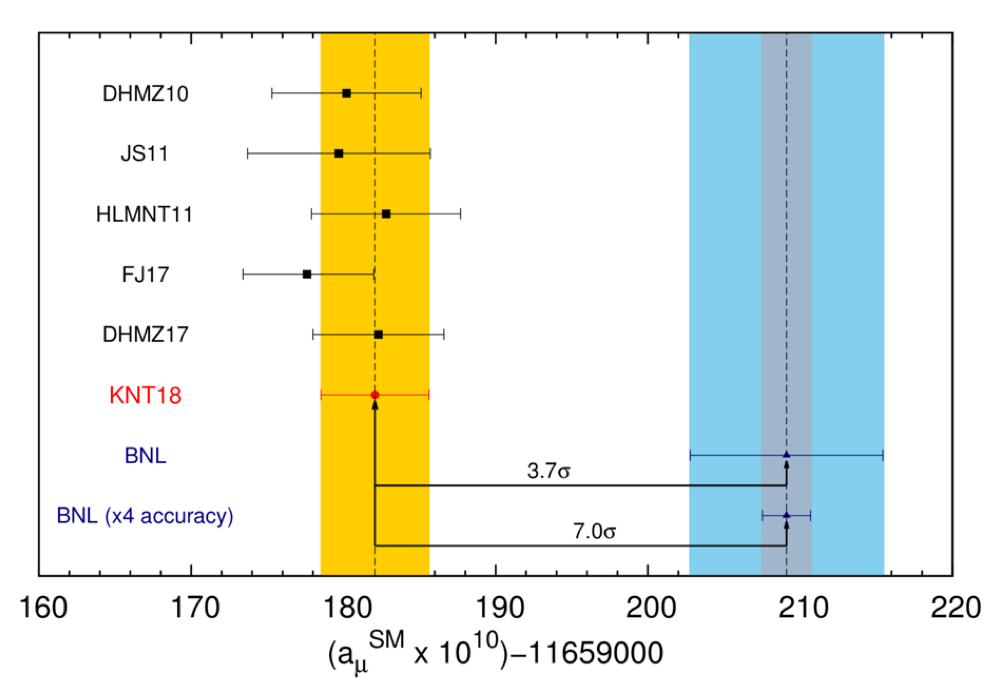
\includegraphics[width=0.9\textwidth]{AlexKPaperComparison}
	\caption[AlexKPaperComparison]{any figures that are directly lifted from someone else's work needs to be cited evertime they're used I believe, even if I cite that work in the text somewhere - \cite{Keshavarzi:2018mgv} }
\end{figure}

Feynamn diagrams made with \cite{tikz-feynman}, \cite{tikz-feynhand}.

\begin{figure}[]
\label{fig:feyn1}
\centering
	\begin{subfigure}[]{0.4\textwidth}
	\centering
		\begin{tikzpicture}[baseline=(o.base)]
		\begin{feynhand}
		\large
		\setlength{\feynhandlinesize}{1pt}
		\vertex [dot] (o) at (0,0);
		\vertex (a) at (-2,-2) {$l$}; 
		\vertex (b) at (2,-2) {$\overline l$}; 
		\vertex (c) at (0,2) {B};
		\propag [fermion] (a) to (o);
		\propag [anti fermion] (b) to (o);
		\propag [photon] (c) to [edge label = $\gamma$] (o);
		\end{feynhand}
		\end{tikzpicture}
	\caption{test1}
	\end{subfigure}
	\begin{subfigure}[]{0.4\textwidth}
	\centering
		\begin{tikzpicture}[baseline=(o.base)]
		\begin{feynhand}
		\large
		\setlength{\feynhandlinesize}{1pt}
		\vertex [dot] (o) at (0,0);
		\vertex (a) at (-2,-2) {$l$}; 
		\vertex (b) at (2,-2) {$\overline l$}; 
		\vertex (c) at (0,2) {B};
		\vertex (d) at (-1,-1);
		\vertex (e) at (1,-1);
		\propag [fermion] (a) to (d);
		\propag [fermion] (d) to (o);
		\propag [anti fermion] (b) to (e);
		\propag [anti fermion] (e) to (o);
		\propag [photon] (c) to [edge label = $\gamma$] (o);
		\propag [photon] (d) to [edge label' = $\gamma$] (e);
		\end{feynhand}
		\end{tikzpicture}
	\caption{test2}
	\end{subfigure}
\caption[testfeynmanpicture2]{clean up and possibly replace - cite this package if I end up using it}	
\end{figure}





\subsection{QED}
\label{subsec:QED}

\subsection{Weak}
\label{subsec:Weak}


\begin{figure}[]
\label{fig:feyn1}
\centering
	\begin{subfigure}[]{0.3\textwidth}
	\centering
		\begin{tikzpicture}[baseline=(o.base)]
		\begin{feynhand}
		\large
		\setlength{\feynhandlinesize}{1pt}
		\vertex [dot] (o) at (0,0);
		\vertex (a) at (-2,-2) {$l$}; 
		\vertex (b) at (2,-2) {$\overline l$}; 
		\vertex (c) at (0,2) {B};
		\vertex (d) at (-1,-1);
		\vertex (e) at (1,-1);
		\propag [fermion] (a) to (d);
		\propag [fermion] (d) to (o);
		\propag [anti fermion] (b) to (e);
		\propag [anti fermion] (e) to (o);
		\propag [photon] (c) to [edge label = $\gamma$] (o);
		\propag [boson] (d) to [edge label' = $Z^{0}$] (e);
		\end{feynhand}
		\end{tikzpicture}
	\caption{test2}
	\end{subfigure}
	\begin{subfigure}[]{0.3\textwidth}
	\centering
		\begin{tikzpicture}[baseline=(o.base)]
		\begin{feynhand}
		\large
		\setlength{\feynhandlinesize}{1pt}
		\vertex [dot] (o) at (0,0);
		\vertex (a) at (-2,-2) {$l$}; 
		\vertex (b) at (2,-2) {$\overline l$}; 
		\vertex (c) at (0,2) {B};
		\vertex (d) at (-1,-1);
		\vertex (e) at (1,-1);
		\propag [fermion] (a) to (d);
		\propag [anti fermion] (b) to (e);
		\propag [photon] (c) to [edge label = $\gamma$] (o);
		\propag [fermion] (d) to [edge label' = $\overline \nu_{l}$] (e);
		\small
		\propag [boson] (d) to [edge label = $W^{-}$] (o);
		\propag [boson] (e) to [edge label' = $W^{+}$] (o);
		\end{feynhand}
		\end{tikzpicture}
	\caption{test2}
	\end{subfigure}
	\begin{subfigure}[]{0.3\textwidth}
	\centering
		\begin{tikzpicture}[baseline=(o.base)]
		\begin{feynhand}
		\large
		\setlength{\feynhandlinesize}{1pt}
		\vertex [dot] (o) at (0,0);
		\vertex (a) at (-2,-2) {$l$}; 
		\vertex (b) at (2,-2) {$\overline l$}; 
		\vertex (c) at (0,2) {B};
		\vertex (d) at (-1,-1);
		\vertex (e) at (1,-1);
		\propag [fermion] (a) to (d);
		\propag [fermion] (d) to (o);
		\propag [anti fermion] (b) to (e);
		\propag [anti fermion] (e) to (o);
		\propag [photon] (c) to [edge label = $\gamma$] (o);
		\propag [scalar] (d) to [edge label' = $H$] (e);
		\end{feynhand}
		\end{tikzpicture}
	\caption{test2}
	\end{subfigure}




	\begin{subfigure}[]{0.4\textwidth}
	\centering
		\begin{tikzpicture}[baseline=(o.base)]
		\begin{feynhand}
		\large
		\setlength{\feynhandlinesize}{1pt}
		\vertex [dot] (o) at (0,0);
		\vertex (a) at (-2,-2) {$l$}; 
		\vertex (b) at (2,-2) {$\overline l$}; 
		\vertex (c) at (0,2) {B};
		\vertex (d) at (-1,-1);
		\vertex (e) at (1,-1);

		\vertex (f) at (-.5,-1);
		\vertex (g) at (+.5,-1);

		\propag [fermion] (a) to (d);
		\propag [fermion] (d) to (o);
		\propag [anti fermion] (b) to (e);
		\propag [anti fermion] (e) to (o);
		\propag [photon] (c) to [edge label = $\gamma$] (o);
		
		\small
		\propag [boson] (d) to [edge label' = $Z^{0}$] (f);
		\propag [boson] (g) to (e);
		\propag [fermion] (f) to [half left, edge label = $f$] (g);
		\propag [anti fermion] (f) to [half right, edge label' = $\overline f$] (g);




		\end{feynhand}
		\end{tikzpicture}
	\caption{test2}
	\end{subfigure}


\caption[testfeynmanpicture2]{clean up and possibly replace - cite this package if I end up using it}	
\end{figure}





\subsection{Hadronic}
\label{subsec:Hadronic}

\subsection{BSM}
\label{subsec:BSM}
